\chapter{Modelado analítico de la PCC \label{chap:ModeloPCC}}
\noindent Además de los sesgos que añaden el fondo y el umbral utilizado sobre la determinación de las magnitudes del factor de Fano y la energía de creación electrón hueco, la colección parcial de carga y la eficiencia de colección de carga juegan un rol fundamental en la determinación precisa de estas magnitudes. Particularmente apreciable es el efecto de estos fenómenos para las mediciones de flúor y aluminio, donde la tasa de eventos es mucho menor a la que se obtuvo en los trabajos previos\cite{TesisAndi,TesisKevin,Rodrigues} con el hierro.
%%%%%%%%%%%%%%%%%%%%%%%%%%%%%%%%%%%%%%%%%%%%%%%%%%%%%%%%%%%%%%%%%%
%%%%%%%%%%%%%%%%%%%%%%%%%%%%%%%%%%%%%%%%%%%%%%%%%%%%%%%%%%%%%%%%%%
\section{Introducción del modelo}
\noindent La física detrás de ellos puede comenzar a modelarse estudiando la distancia que recorren los fotones dentro del material del sensor hasta que interactúan con él. Esta es una variable aleatoria de distribución exponencial, que viene dada por
\begin{equation}
    f_{Z}(z) = \frac{1}{\tau_{\scaleto{X}{4pt}}}\exp(-\frac{z}{\tau_{\scaleto{X}{4pt}}})
        \label{ec:DistribucionDistancias}
\end{equation}
donde $\tau_{\scaleto{X}{4pt}}$ es la longitud de atenuación, que es la distancia promedio para la cual la cantidad de fotones incidentes se reduce a una fracción de $1/e$ de la población original. Este es un valor tabulado tanto para la energía de los fotones como para el material. Para el caso del silicio, puede verse en el gráfico de la figura \ref{fig:Attenuation} la relación entre la longitud de atenuación $\tau_{\scaleto{X}{4pt}}$ y la energía de un fotón incidente. Por ejemplo, para el caso de la energía correspondiente a los rayos $X$ del flúor, $677\,\si{eV}$, se tiene que la longitud de atenuación es aproximadamente $1\,\si{\mu m}$, mientras que para los rayos $X$ del aluminio, $\sim 1500\,\si{eV}$, la longitud de atenuación ronda los $8\,\si{\mu m}$.
\begin{figure}[h]
    \centering
        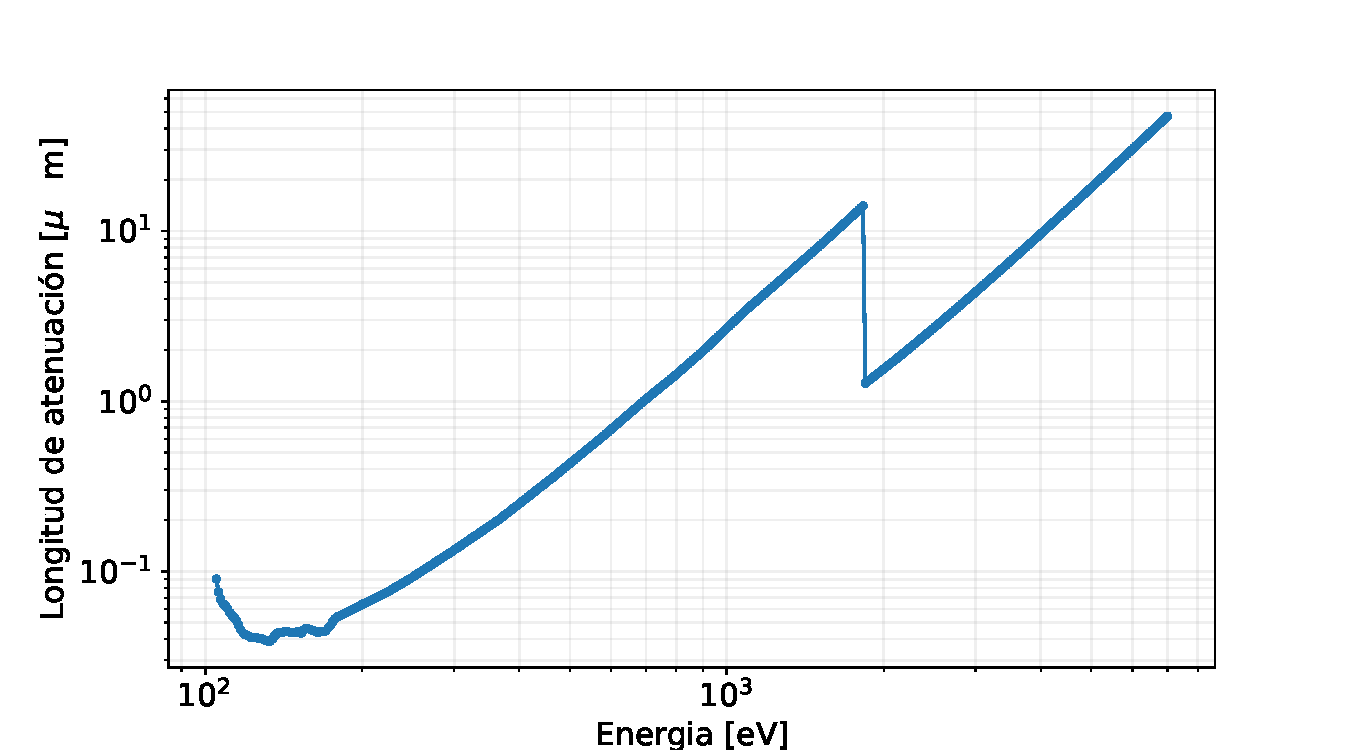
\includegraphics[scale=0.5]{Figs/AttenuationLength.pdf}
    \caption{\footnotesize{Longitud de atenuación para el silicio en función de la energía de un fotón que incide con un ángulo de $90\,^{\circ}$ sobre el material. Datos obtenidos de \textit{The Center for X-Ray Optics}\cite{AttenuationLength}.}}
    \label{fig:Attenuation}
\end{figure}
Realizaciones de la variable aleatoria de esta distribución son las diferentes distancias que puede alcanzar un fotón que penetra en el sensor hasta generar cargas por ionización.

Por otro lado, se puede caracterizar la eficiencia de colección de carga con una función para la cual a una dada distancia de penetración $z$ se tiene qué fracción de la carga inicial logra ser colectada. Dicha función viene dada por
\begin{equation}
    E_{ff}(z) = 1 - 
    \exp
    \left(
        -\frac{z}{\tau_{\scaleto{CCE}{4pt}}}
    \right)
        \label{ec:funcionCCE}
\end{equation}
donde $\tau_{\scaleto{CCE}{4pt}}$ es la distancia media para la cual la cantidad de carga ionizada que sufre recombinación cae a $1/e$ del total de carga inicial. En el gráfico de la figura \ref{fig:EficienciaCC} se ven los datos obtenidos de mediciones realizadas utilizando el pico de los rayos $X$ del flúor y su ajuste a partir del uso de esta función.
\begin{figure}[H]
    \centering
        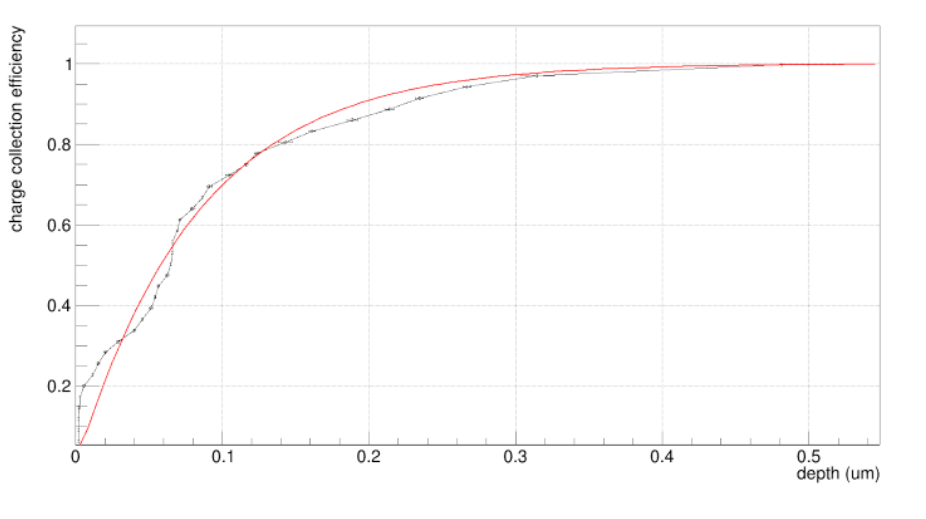
\includegraphics[scale=0.3]{pngs/CCE_plot.png}
    \caption{\footnotesize{Mediciones de la eficiencia de colección de carga como función de la profundidad y ajuste de los mismos utilizando la función de eficiencia de la colección de carga. Datos obtenidos de mediciones con rayos $X$ del flúor de $677\,\si{eV}$. Se ve como luego de los primeros $\sim 400\,\si{nm}$ ya es colectada casi el $100\,\%$ de la carga producida por ionización.}}
    \label{fig:EficienciaCC}
\end{figure}
Se busca combinar ambas expresiones, donde la primera de ellas es una distribución y describe un proceso estocástico mientras que la segunda es una función convencional. Para esto es necesario lograr incorporar la variable aleatoria $z$, que viene de la distribución \ref{ec:DistribucionDistancias}, dentro de la función de eficiencia \ref{ec:funcionCCE}, de modo de obtener una nueva distribución $f_{E_{ff}}$ para la eficiencia o probabilidad de colectar carga. La nueva variable $\varepsilon$ tiene una dependencia funcional conocida y es $\varepsilon = \varepsilon(z)$ y viene definida por $E_{ff}(z) = \varepsilon$. En este sentido, dada una correspondencia uno a uno entre la vieja y la nueva variable, la probabilidad en un intervalo diferencial tiene que conservarse, con lo cual, dada la distribución $f_{Z}(z)$ inicial y la distribución final $f_{E_{ff}}(\varepsilon)$, tiene que valer que
\begin{equation*}
    f_{Z}(z)\,dz = f_{E_{ff}}(\varepsilon)\,d\varepsilon
\end{equation*}
de esta forma se puede escribir $f_{E_{ff}}$ en términos de la distribución inicial como sigue
\begin{equation*}
    f_{E_{ff}} 
    = f_{Z}
    \left|
        \frac{dz}{d\varepsilon}
    \right|
\end{equation*}
Donde aparece un Jacobiano y se agrega el módulo para asegurar una dependencia no negativa. Como la nueva variable $\varepsilon$ es función de $z$, $E_{ff}(z) = \varepsilon$, entonces $E_{ff}^{-1}(\varepsilon) = z$ y se puede escribir la última en términos de $\varepsilon$
\begin{equation*}
    f_{E_{ff}}(\varepsilon) 
    = f_{Z}
    \left(
        E_{ff}^{-1}(\varepsilon)
    \right)
    \left|
        \frac{dE_{ff}^{-1}(\varepsilon)}{d\varepsilon}
    \right|
\end{equation*}
finalmente, resolviendo esta última se obtiene la expresión para la nueva distribución, que resulta ser una Beta de parámetro $\alpha = 1$ y $\beta$ libre.
\begin{equation*}
    f_{E_{ff}}(\varepsilon) = \beta (1 - \varepsilon)^{\beta - 1}
\end{equation*}
donde además se definió el parámetro $\beta$ como $\beta = \frac{\tau_{\scaleto{CCE}{3pt}}}{\tau_{\scaleto{X}{3pt}}}$. Esta es la distribución de probabilidad de colectar la carga producida por un fotón de una dada energía y puede verse un ejemplo de ajuste a un conjunto de datos simulados con esta distribución en la figura \ref{fig:BetaDistyAjuste}.
\begin{figure}[h]
    \centering
        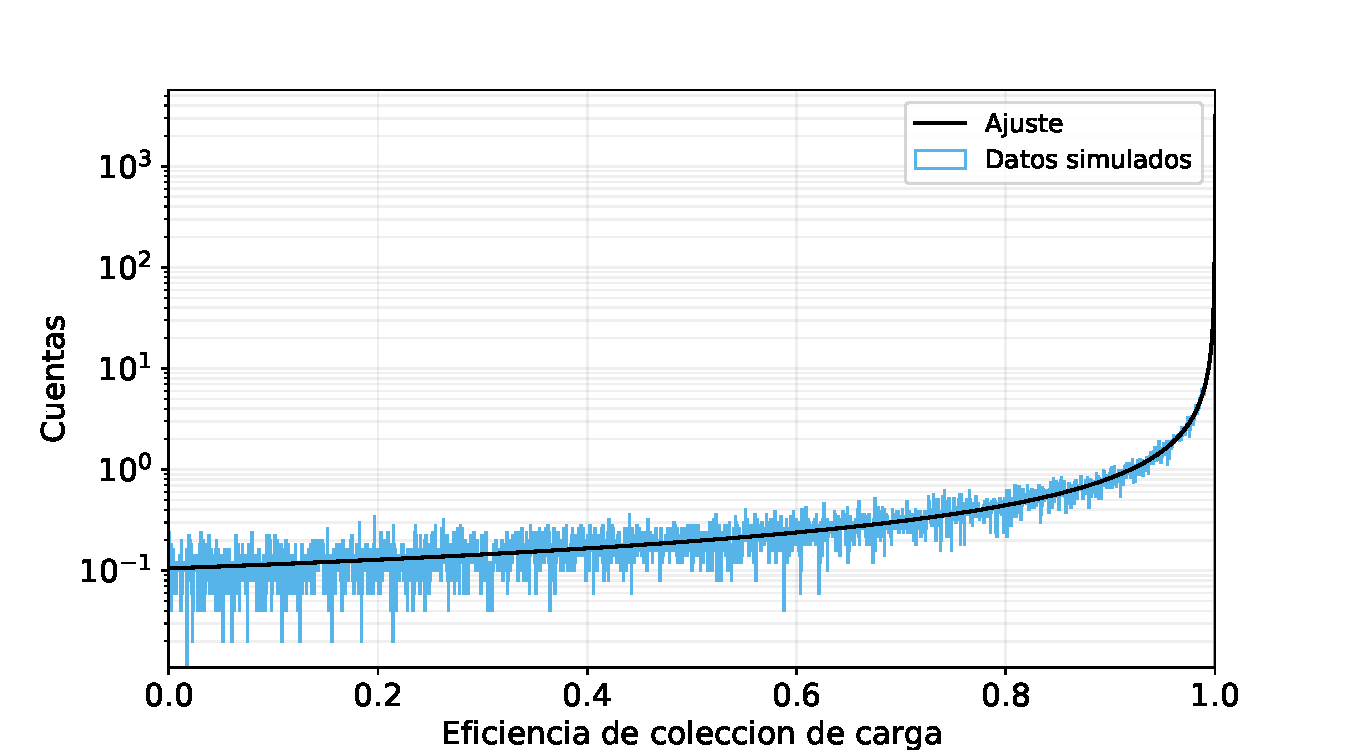
\includegraphics[scale=0.5]{Figs/BetaDistyAjuste.pdf}
    \caption{\footnotesize{Distribución de la eficiencia de colección de carga obtenida de un simulación \textit{toy} Monte-Carlo (histograma) y su ajuste con el modelo descripto (trazo continuo).}}
    \label{fig:BetaDistyAjuste}
\end{figure}

Sin embargo, para terminar de modelar todos los efectos que contribuyen a la dispersión de la carga generada por ionización en el material, hay que considerar que, además de los efectos anteriores, para una dada energía no siempre se producirán la misma cantidad de carga, efecto descripto por el factor de Fano. Dado que cada proceso de ionización puede considerarse como un experimento de Bernoulli, una sucesión de interacciones puede pensarse como un fenómeno binomial. En el límite, donde la probabilidad de ionización es baja y la cantidad de veces que puede haber interacciones es muy alta, el proceso se vuelve Poissoniano. Cuando la esperanza de dicha distribución es alta (mayor a $100$ en los casos de interés en este trabajo), el límite gaussiano dado por el teorema central del límite se cumple en excelente aproximación. Con lo cual, la distribución de carga para los eventos de interés puede modelarse sin perder precisión con una distribución gaussiana de la siguiente forma
\begin{equation*}
    f_{Q_{i}}(q_{i}) = 
    \frac{1}{\sqrt{2\pi \sigma^{2}}}\,
    \exp
        \left[
            -\frac{1}{2}
            \left(
                \frac{q_{i} - \mu}{\sigma}
            \right)^{2}
        \right]
\end{equation*}
donde $q_{i}$ es la cantidad de carga inicial ionizada. Para agregar esta última contribución al modelado del fenómeno, combinando todas las contribuciones, es necesario realizar la convolución de ambas distribuciones: la distribución de probabilidad de colectar carga dada una distancia de penetración $z$ y la distribución de probabilidad de generar carga dada una energía inicial. Entonces, se escribe la probabilidad unión de ambas como
\begin{equation*}
    f_{Q_{i} \times E_{ff}} (q_{i}, \varepsilon)
    \equiv f_{Q_{i}}(q_{i}) f_{E_{ff}}(\varepsilon)
    =
    \frac{1}{\sqrt{2\pi \sigma^{2}}}
    \exp
        \left[
            -\frac{1}{2}
            \left(
                \frac{q_{i} - \mu}{\sigma}
            \right)^{2}
        \right]
    \beta(1-\varepsilon)^{\beta - 1}
\end{equation*}
Se busca obtener una nueva distribución $f_{Q_{f}\times E_{ff}}$ para la carga $q_{f}$ que logra escapar de la región de PCC, sin embargo la expresión anterior está escrita en función de la carga ionizada inicial, $q_{i}$. Notando que existe una relación funcional entre ambas que se obtiene a partir de la eficiencia $\varepsilon$ como
\begin{equation*}
    \varepsilon = \frac{q_{f}}{q_{i}}
    \Longrightarrow
    q_{f} = q_{f}(q_{i}),
\end{equation*}
se puede realizar un cambio de variables para obtener la nueva distribución, siempre y cuando la nueva y la vieja distribución cumplan que
\begin{equation*}
    f_{Q_{f}\times E_{ff}}(q_{f}, \varepsilon)\,dq_{f} =
    f_{Q_{i}\times E_{ff}}(q_{i}, \varepsilon)\,dq_{i}
\end{equation*}
de donde puede obtenerse una expresión para $f_{Q_{f}\times E_{ff}}$ y que escribiendo explícitamente $f_{Q_{i}\times E_{ff}}$ resulta de la forma
\begin{equation*}
    f_{Q_{f}\times E_{ff}}(q_{f}, \varepsilon)
    = 
    \frac{1}{\sqrt{2\pi \sigma^{2}}}
    \exp
        \left[
            -\frac{1}{2}
            \left(
                \frac{q_{i} - \mu}{\sigma}
            \right)^{2}
        \right]
    \beta(1-\varepsilon)^{\beta - 1}
    \left|
        \frac{dq_{i}}{dq_{f}}
    \right|
\end{equation*}
donde se ha agregado un módulo al Jacobiano para asegurar la positividad, sin embargo en este caso en particular no resultará necesario. 

Como $q_{i} = q_{f}/\varepsilon$, y la eficiencia $\varepsilon > 0$, en particular $\varepsilon \in [0, 1]$ entonces se tiene que 
\begin{equation*}
    \left|
        \frac{dq_{i}}{dq_{f}}
    \right|
        = 
    \left|
        \frac{d}{dq_{f}}
        \left(
            \frac{q_{f}}{\varepsilon}
        \right)
    \right|
        = 
        \frac{1}{\varepsilon}
\end{equation*}
reemplazando esto último y acomodando términos se obtiene la distribución de probabilidad unión como
\begin{equation*}
    f_{Q_{f}\times E_{ff}}(q_{f})
    = 
    \frac{1}{\sqrt{2\pi \sigma^{2}\varepsilon^{2}}}
    \exp
        \left[
            -\frac{1}{2}
            \left(
                \frac{q_{f} - \varepsilon\mu}{\varepsilon\sigma}
            \right)^{2}
        \right]
    \beta(1-\varepsilon)^{\beta - 1}
\end{equation*}
finalmente, integrando respecto de $\varepsilon$ para obtener la distribución de $q_{f}$ se llega a la expresión final del modelo,
\begin{equation}
    f_{Q_{f}}(q_{f}) = 
    \int\limits_{0}^{1}
    \frac{\beta(1-\varepsilon)^{\beta - 1}}{\sqrt{2\pi \sigma^{2}\varepsilon^{2}}}
    \exp
        \left[
            -\frac{1}{2}
            \left(
                \frac{q_{f} - \varepsilon\mu}{\sigma\varepsilon}
            \right)^{2}
        \right]\,
    d\varepsilon
    \label{ec:UnbinnedFit}
\end{equation}
el cual fue específicamente construido para la distribución teórica de carga debido a los efectos del factor de Fano y la colección parcial de carga actuando conjuntamente. Por otro lado, no se logró encontrar una expresión analítica para la solución de esta integral, con lo cual es necesario resolverla numéricamente.

%%%%%%%%%%%%%%%%%%%%%%%%%%%%%%%%%%%%%%%%%%%%%%%%%%%%%%%%%%%%%%%%%%
%%%%%%%%%%%%%%%%%%%%%%%%%%%%%%%%%%%%%%%%%%%%%%%%%%%%%%%%%%%%%%%%
\section{Máxima verosimilitud y determinación del intervalo de \texorpdfstring{$\beta$}{beta}\label{sec:MaximaVerosimilitud}}
\noindent Para obtener los parámetros $\mu$, $\sigma$ y $\beta$ del modelo lo que se hace es fijar un valor para el parámetro $\beta$ y luego ajustar los datos para obtener $\mu$ y $\sigma$. Una vez ajustados estos parámetros, se calcula la verosimilitud a partir de la distribución de probabilidad resultante. Realizando un barrido en valores del parámetro $\beta$ se obtienen diferentes ajustes y a su vez diferentes valores de la verosimilitud resultante para cada $\beta$. De esta forma, se busca el $\hat{\beta}$ que maximiza el valor de la verosimilitud y de ese ajuste se obtienen los parámetros $\mu$ y $\sigma$ óptimos. Los errores para $\mu$ y $\sigma$ se obtienen directamente del ajuste. 

Por otro lado, debido a que el efecto que introduce en las mediciones la colección parcial de carga es pequeño, se espera que la estadística sea baja en las colas de los picos. Es por esa razón que el análisis de la incerteza del parámetro $\beta$ requiere del uso de otras herramientas de cálculo, en particular, esta se obtiene gráficamente de la curva de la verosimilitud. Se busca el intervalo de confianza de la verosimilitud de $68.3\,\%$ de probabilidad que contenga al parámetro $\beta$. Para obtener este intervalo, lo que se debe hacer es tomar el máximo valor del logaritmo de la verosimilitud en función de $\beta$ y obtener la intersección de la parábola formada por esta con una recta que se encuentra a una distancia $a$ por debajo del máximo, donde $a = 1/2$, es decir, los valores 
\begin{equation*}
    \left\{
        \beta\ \in\ \mathbb{R}\ /\ 
        \ln{(L(\hat{\beta}))}
        -
        \ln{
            \left(
                L(\beta)
            \right)
            }
        = 1/2
    \right\}
\end{equation*}
Los $\beta$ donde la recta y la parábola se tocan corresponden a los límites izquierdos y derechos del intervalo de $68.3\,\%$ deseado\cite{Frodesen}.

%%%%%%%%%%%%%%%%%%%%%%%%%%%%%%%%%%%%%%%%%%%%%%%%%%%%%%%%%%%%%%%%%%%%
%%%%%%%%%%%%%%%%%%%%%%%%%%%%%%%%%%%%%%%%%%%%%%%%%%%%%%%%%%%%%%%%%%
\section{Características del modelo}
\noindent Utilizar este modelo para ajustar los picos de los histogramas de carga tiene la ventaja de que los parámetros que se obtienen del ajuste, como el valor medio $\mu$ y su dispersión $\sigma$, son los valores que se obtendrían si la colección parcial de carga fuera totalmente nula. Es decir, este modelo logra obtener estas magnitudes disociando totalmente el efecto de la PCC. A su vez, también se obtiene el parámetro $\beta$, el cual venía definido como la relación entre $\tau_{\scaleto{CCE}{4pt}}$ y $\tau_{\scaleto{X}{4pt}}$, donde el primero es un parámetro intrínseco del material del detector y, por ende, está fijo, mientras que el segundo es una magnitud que varía dependiendo de la energía incidente y del material. Más aún, $\tau_{\scaleto{CCE}{4pt}}$ puede definirse como el ancho de la región de colección parcial de carga del detector, de forma que obteniendo $\beta$ a partir de un ajuste del modelo y $\tau_{\scaleto{X}{4pt}}$ a partir de tablas, se puede saber el tamaño de la región de PCC. Con lo cual, este modelo es capaz de determinar el espesor de la región del sensor donde hay probabilidad de tener recombinación de carga.

También es importante destacar que este modelo se enfoca en capturar el efecto que provoca la colección parcial de carga en los picos de los histogramas, pero ignora otros fenómenos que en general podrían introducir fondo, como ser la dispersión por efecto Compton o la generación de pares. Esto se debe a que en las escalas de energía en las que se trabajó, los efectos de estos fenómenos son despreciables o, más aún, imposibles para el caso de generación de pares. 
\begin{figure}[h]
    \centering
        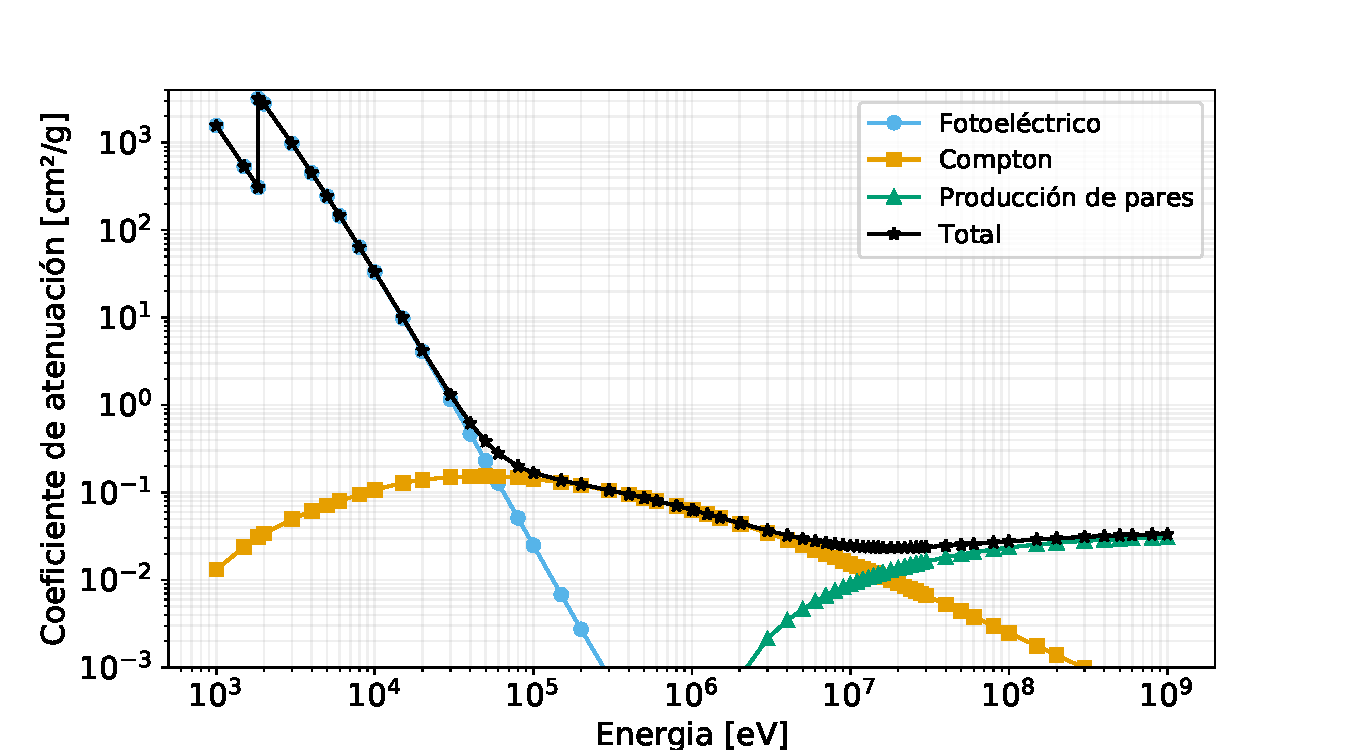
\includegraphics[scale=0.5]{Figs/FotoelectricoComptonPares_enSilicio.pdf}
    \caption{\footnotesize{Diferentes contribuciones al coeficiente de atenuación del Silicio. Se observa que el efecto fotoeléctrico es la contribución preponderante en los órdenes de energía estudiados en este trabajo.}}
    \label{fig:FotoelectricoComptonPares}
\end{figure}
En el gráfico de la figura \ref{fig:FotoelectricoComptonPares} se encuentran las curvas de los coeficientes de atenuación para el silicio dependiendo del tipo de proceso de dispersión, obtenidas del \textit{National Institute of Standards and Technology}\cite{FotoComptPar}, como ser, el efecto fotoeléctrico, el efecto Compton, la generación de pares y la suma de los tres efectos. Se observa de la figura \ref{fig:FotoelectricoComptonPares} que para energías menores a los $1000\,\si{eV}$ la contribución del efecto Compton es totalmente despreciable frente a la del efecto fotoeléctrico, la cual domina en todo el rango de energías de estudiado en este trabajo.

Resulta importante notar que, debido a que la longitud de atenuación $\tau_{\scaleto{X}{4pt}}$ depende de la energía del fotón incidente (entre otros), para el caso de los rayos $X$ del flúor cuya energía es menor a la de los rayos $X$ del aluminio, la longitud de atenuación es menor. Por otro lado, como $\tau_{\scaleto{CCE}{4pt}}$ es una característica del detector y no depende de ningún parámetro, y como $\beta = \tau_{\scaleto{CCE}{4pt}}/\tau_{\scaleto{X}{4pt}}$, entonces se espera que el valor de $\beta$ sea mucho mayor en el caso del flúor respecto del aluminio. Con lo cual, el efecto de la colección parcial carga debería ser más pronunciado en esos picos. Esto implica que debería poder apreciarse colas más pronunciadas a la izquierda de los picos para dicho material.

%\indent Si el detector fuera perfecto, el factor de Fano existiría igual. Este no es un problema del detector, viene del proceso de interacción en sí mismo que a la larga es un fenómeno binomial. Sin embargo, lo que sí es un problema del detector es la PCC. Un fotón interactuando con materia es un experimento Bernoulli, una serie de procesos de interacción es un fenómeno binomial y, en consecuencia, en el límite de probabilidades pequeñas y gran número de repeticiones, de Poisson. Por lo tanto, cuán lejos llega es una variable aleatoria con distribución exponencia (La distancia entre dos eventos de poisson es exponencial). Si uno quiere saber cuál es la probabilidad de que un fotón penetre una dada distancia, hay que hacer
%\begin{equation*}
%    e^{-\frac{d}{\tau}}
%\end{equation*}
%con $\tau$ es la attenuation length. La eficiencia de colección de carga viene dada por 
%\begin{equation*}
%    E_{ff}(z) = 1 - e^{-\frac{z}{\tau_{\scaleto{CEE}{2pt}}}}
%\end{equation*}
%que quiere decir que si la interacción se realizó para un dado $z_{0}$, entonces por ejemplo el $70\%$ de la carga logró ser colectada. Para $Z_{0}$ muy chico, la eficiencia es muy chica, para $z_{0}$ creciente, la eficiencia es creciente.

%Dada la variable aleatoria: Longitud penetrada hasta interactuar, tiene una distribución exponencial. Dada una energía fija, la longitud que recorre hasta interactuar no es siempre la misma, hay una aleatoria inherente. La distribución de probabilidades de este experimento es exponencial. Si por ejemplo la probabilidad de interactuar en los primeros $3\,\si{\mu m}$ es del $50\%$, la probabilidad de interactuar recién luego de recorridos $80\,\si{\mu m}$ es $10^{-14}$. Esta variable aleatoria se inyecta dentro de la función $E_{ff}(z)$: Función a la que le digo hasta donde llegó la partícula antes de interactuar y devuelve con qué eficiencia colectó la carga.

%Se tiene la energía del fotón, se genera un evento aleatorio con distribución exponencial $z_{0}$ que dice qué distancia penetró el fotón antes de interactuar. Esa realización se usa como argumento de $E_{ff}(z) \longrightarrow E_{ff}(z_{0})$. Ese cambio de variables da como resultado 
%\begin{equation*}
%    f_{E_{ff}}(z) = \beta (1 - \varepsilon)^{\beta - 1}
%\end{equation*}
%donde $\beta = \frac{\tau_{\scaleto{CCE}{3pt}}}{\tau_{\scaleto{X}{3pt}}}$. La probabilidad de recuperar la carga de un fotón de una dada energía sigue esa distribución.

%Todavía no entró el Fano. A esto hay que agregarle que además de haber una distribución de carga para la profundidad, además de haber una función que dice cuánta carga se logra colectar con esa profundidad, hay otra variable aleatoria que es cuántos electrones se ionizan cuando se interactúa, que viene de una poissoniana, pero en el límite se puede pensar como una gaussiana. Entonces, a la función anterior hay que convolucionarla con una gaussiana. El efecto de convolucionar una gaussiana con esta distribución es añadirle una cola del lado izquierdo a la gaussiana. De hacer esa convolución se obtiene
%\begin{equation*}
%     f_{Q_{f}}(q_{f}) = 
%     \int\limits_{0}^{1}
%     \frac{\beta}{\sqrt{2\pi \sigma^{2}}\varepsilon}
%     \exp[%
%     -\frac{(q_{f}-\varepsilon\mu)^{2}}{2\sigma^{2}\varepsilon^{2}}
%     ](1-\varepsilon)^{\beta - 1}
%     d\varepsilon
% \end{equation*}
%La cola que aparece a la izquierda es culpa de la PCC, debido a que hay eventos con menor carga generada debido a este fenómeno de recombinación para los eventos que suceden en los primeros micrones del detector. Del lado derecho no hay nada porque no hay un fenómeno que genere más carga de la que el proceso de ionización puede generar.
%%%%%%%%%%%%%%%%%%%%%%%%%%%%%%%%%%%%%%%%%%%%%%%%%%%%%%%%%%%%%%%%%%
%%%%%%%%%%%%%%%%%%%%%%%%%%%%%%%%%%%%%%%%%%%%%%%%%%%%%%%%%%%%%%%%%%
